\documentclass[10pt]{article}
\usepackage[paperwidth=594mm,paperheight=420mm,margin=15mm,top=13mm,bottom=11mm]{geometry}
\usepackage[T1]{fontenc}
\usepackage[utf8]{inputenc}
\usepackage{lmodern}
\usepackage{microtype}
\usepackage{amsmath,amssymb,mathtools}
\usepackage{graphicx}
\usepackage{xcolor}
\usepackage{tikz}
\usepackage[most]{tcolorbox}
\usepackage{tabularx,booktabs,array}
\usepackage{enumitem}
\usepackage{ragged2e}
\usepackage{hyperref}
\usepackage{titlesec}
\usepackage{fancyhdr}
\usepackage{calc}
\usepackage{ ctex}
\definecolor{Ink}{HTML}{182B3A}
\definecolor{Navy}{HTML}{24465A}
\definecolor{Teal}{HTML}{397C78}
\definecolor{Orange}{HTML}{D77A42}
\definecolor{Badge}{HTML}{E4572E}
\definecolor{Paper}{HTML}{F5F3EE}
\definecolor{Mist}{HTML}{E9EFED}
\definecolor{Line}{HTML}{D8DCD8}
\definecolor{Muted}{HTML}{68757A}
\color{Ink}
\hypersetup{colorlinks=true,linkcolor=Navy,urlcolor=Teal,citecolor=Teal,
	pdftitle={Hydrodynamics of the Viscous Electron Fluid in Cadmium},
	pdfauthor={X. Guo, X. Li, B. Fauque, A. Subedi, L. Zhao, Z. Zhu, K. Behnia},
	pdfsubject={Phys. Rev. Lett. 137, 206301 (2026); DOI: 10.1103/g32f-j6q2},
	pdfcreator={A Travelling Snail},
	pdfkeywords={electron hydrodynamics, Gurzhi effect, cadmium, electron viscosity}}
\setlength{\parindent}{0pt}
\setlength{\parskip}{3pt}
\setlength{\abovedisplayskip}{1.5pt plus 0.5pt minus 0.5pt}
\setlength{\belowdisplayskip}{1.5pt plus 0.5pt minus 0.5pt}
\setlength{\abovedisplayshortskip}{1pt}
\setlength{\belowdisplayshortskip}{1pt}
\setlist[itemize]{leftmargin=1.1em,itemsep=3pt,topsep=2pt,parsep=0pt}
\setlist[enumerate]{leftmargin=1.3em,itemsep=2.5pt,topsep=2pt}
\renewcommand{\arraystretch}{1.15}
\setlength{\tabcolsep}{4pt}

\newcommand{\eyebrow}[1]{{\sffamily\bfseries\fontsize{9.7}{11.8}\selectfont\color{Teal}\MakeUppercase{#1}}}
\newcommand{\sectionhead}[2]{\vspace{1pt}{\eyebrow{#1}\hspace{6pt}{\color{Orange}\rule{1.4em}{1.2pt}}}\par\vspace{2pt}{\sffamily\bfseries\fontsize{14.2}{16.5}\selectfont\color{Ink}#2}\par\vspace{3pt}}
\newcommand{\smallnote}[1]{{\fontsize{9.4}{11.3}\selectfont\color{Muted}#1}}
\newcommand{\papertag}[1]{\leavevmode\colorbox{Mist}{\strut\hspace{4pt}\fontsize{9.4}{11.3}\selectfont\sffamily\color{Navy}#1\hspace{4pt}}}

\tcbset{enhanced,boxrule=0pt,arc=1.5mm,left=7pt,right=7pt,top=5pt,bottom=5pt}
\newtcolorbox{takeawaybox}{colback=Paper}
\newtcolorbox{equationbox}{colback=Mist}
\newtcolorbox{questionbox}{colback=Paper,borderline west={2.2pt}{0pt}{Orange}}
\newtcolorbox{figurebox}{colback=Paper,boxsep=2pt,left=4pt,right=4pt,top=4pt,bottom=4pt}
\newtcolorbox{regimeNavy}{colback=Paper,boxrule=0pt,arc=1mm,left=7pt,right=7pt,top=3pt,bottom=3pt,
	borderline west={2.4pt}{0pt}{Navy},fontupper=\fontsize{10.6}{13.2}\selectfont}
\newtcolorbox{regimeTeal}{colback=Paper,boxrule=0pt,arc=1mm,left=7pt,right=7pt,top=3pt,bottom=3pt,
	borderline west={2.4pt}{0pt}{Teal},fontupper=\fontsize{10.6}{13.2}\selectfont}
\newtcolorbox{regimeOrange}{colback=Paper,boxrule=0pt,arc=1mm,left=7pt,right=7pt,top=3pt,bottom=3pt,
	borderline west={2.4pt}{0pt}{Orange},fontupper=\fontsize{10.6}{13.2}\selectfont}

% Figure caption: label + bold lead + 3--4 line description
\newcommand{\figcap}[3]{%
	\par\vspace{2.5pt}\begingroup\RaggedRight
	{\fontsize{9.7}{11.5}\selectfont\sffamily\bfseries\color{Navy}#1}\hspace{5pt}%
	{\fontsize{9.7}{11.5}\selectfont\sffamily\bfseries\color{Ink}#2}\par\vspace{1.5pt}%
	{\fontsize{9.2}{11.1}\selectfont\color{Ink}#3\par}%
	\endgroup}

\newcommand{\figpanel}[4][1.0]{%
	\begin{figurebox}\centering
		\includegraphics[width=#1\linewidth]{#2}%
		\figcap{#3}{#4}{}%
	\end{figurebox}}

\pagestyle{empty}
\begin{document}

% ============================================================
% A3 POSTER — landscape 420 x 297 mm
% ============================================================
\noindent{\color{Teal}\rule{\textwidth}{2.2pt}}\par
\vspace{5pt}

\begin{minipage}[b]{0.74\textwidth}
	{\eyebrow{Electronic transport \textbullet\ Hydrodynamics}}\\[1pt]
	{\sffamily\bfseries\fontsize{30.2}{33.5}\selectfont\color{Ink}Hydrodynamics of the Viscous Electron Fluid in Cadmium}\\[3pt]
	{\fontsize{10.9}{13.2}\selectfont\color{Muted}X. Guo, X. Li, B. Fauqu\'e, A. Subedi, L. Zhao, Z. Zhu, K. Behnia\quad\textbullet\quad Phys.\ Rev.\ Lett.\ \textbf{137}, 206301 (2026)\quad\textbullet\quad DOI: \href{https://doi.org/10.1103/g32f-j6q2}{10.1103/g32f-j6q2}}
\end{minipage}\hfill
\begin{minipage}[b]{0.23\textwidth}\raggedleft
	{\colorbox{Badge}{\color{white}\sffamily\bfseries\fontsize{11.8}{14.2}\selectfont\hspace{5pt}MADE BY\quad A TRAVELLING SNAIL\hspace{5pt}}}\\[3pt]
	{\sffamily\bfseries\fontsize{22.4}{24.8}\selectfont\color{Teal} 远行的蜗牛}\\[1pt]
	{\smallnote{Phys.\ Rev.\ Lett.\ \textbf{137} (2026)}}
\end{minipage}

\vspace{5pt}\par{\color{Line}\hrule height 0.7pt}\par
\vspace{7pt}

% ============================================================
% THREE-COLUMN BODY
% ============================================================
\begin{minipage}[t]{0.31\textwidth}\vspace{0pt}\RaggedRight
	\fontsize{10.6}{13.3}\selectfont

					\sectionhead{01 / Three regimes}{Length scale selects transport}
	{\fontsize{10.6}{13.2}\selectfont
	The ratios $s/l_{\mathrm{MC}}$ and $s/l_{\mathrm{MR}}$ select the transport regime.\par}

	\vfill
	\begin{regimeNavy}
		{\sffamily\bfseries\fontsize{13}{15.3}\selectfont\color{Navy}(A)}\quad
		{\sffamily\bfseries\fontsize{11.8}{14.2}\selectfont Diffusive}\hfill
		{\smallnote{bulk scattering}}\par\vspace{1pt}
		\[
			s\gg l_{\mathrm{MR}}>l_{\mathrm{MC}}
			\qquad
			\sigma_{\mathrm{diff}}=\frac{ne^2\tau_{\mathrm{MR}}}{m^*}
		\]
		\[
			\frac{1}{\tau}\propto T^2
			\qquad
			\rho-\rho_0\propto T^2
		\]
		{\fontsize{10.6}{13.2}\selectfont
		In large samples, transport is controlled by bulk momentum-relaxing scattering. Electron--electron Umklapp collisions transfer crystal momentum to the lattice, so the directed motion decays. As $T$ rises and collisions become more frequent, the resistivity increases---conventional Fermi-liquid transport.\par}
	\end{regimeNavy}

	\vfill
	\begin{regimeTeal}
		{\sffamily\bfseries\fontsize{13}{15.3}\selectfont\color{Teal}(B)}\quad
		{\sffamily\bfseries\fontsize{11.8}{14.2}\selectfont Hydrodynamic}\hfill
		{\smallnote{viscous fluid}}\par\vspace{1pt}
		\[
			l_{\mathrm{MC}}<s<l_{\mathrm{MR}}
		\]
		{\fontsize{10.6}{13.2}\selectfont\itshape Local equilibrium---viscous electron fluid.From Navier-Stokes Equation\par}
		\[
			\frac{\partial\mathbf u}{\partial t}
			+\mathbf u\cdot\nabla\mathbf u
			=-\frac{1}{\rho}\nabla P
			+\nu\nabla^2\mathbf u
		\]
		\[
			\mathrm{Re}
			=\frac{U^2/L}{\nu U/L^2}
			=\frac{UL}{\nu}\ll1
		\]
		{\smallnote{Viscous dominated regime.The terms on the right side of the equation are balanced.}}\par\vspace{1pt}
		\[
			\Delta P_x\sim neE
			\sim\eta\frac{\partial^2u}{\partial z^2}
			\qquad
			u(z=0)=0,\quad u(z=s)=0
		\]
		\[
			\bar u=\frac{1}{s}\int_0^s u\,dz
			\propto\frac{E s^2}{\eta}
			\qquad
			j=ne\bar u
			\propto E\frac{s^2}{\eta}
		\]
		\[
			\sigma\propto\frac{s^2}{\eta}
			\propto\frac{s^2}{\nu}
			\qquad
			\nu\sim UL \sim  v_F^2\tau_{\mathrm{MC}}
		\]
		\[\sigma \propto \frac{ s^2}{ v_F^2\tau_{\mathrm{MC}}}\]
		\[
			\frac{1}{\tau}\propto T^2
			\qquad
			\sigma \propto T^2
		\]
		{\fontsize{10.6}{13.2}\selectfont
		In small samples, momentum-conserving electron--electron collisions are frequent enough to establish local equilibrium, forming a viscous electron fluid. Collisions    redistribute momentum internally until it reaches the sample boundaries. Raising $T$ makes these collisions more frequent, shortens the momentum-diffusion length, and lowers the viscosity. Since boundary drag is weakened, the flow becomes smoother, and the conductivity increases (the Gurzhi effect).\par}
	 
	\end{regimeTeal}

	\vfill
	\begin{regimeOrange}
		{\sffamily\bfseries\fontsize{13}{15.3}\selectfont\color{Orange}(C)}\quad
		{\sffamily\bfseries\fontsize{11.8}{14.2}\selectfont Ballistic}\hfill
		{\smallnote{boundary-limited}}\par\vspace{1pt}
		\[
			s\ll l_{\mathrm{MC}}
			\qquad
			v_F\tau\sim s
		\]
		\[
			\rho\propto\frac{1}{\tau}\propto\frac{1}{s}
			\qquad
			\rho\propto T^0
		\]
		{\fontsize{10.6}{13.2}\selectfont
		When the sample is smaller than $l_{\mathrm{MC}}$, electrons cross it before enough momentum-conserving collisions occur, so local equilibrium is not established. Transport is boundary-limited, and the resistivity is temperature-independent.\par}
	\end{regimeOrange}

	
	\vfill
	\begin{takeawaybox}
		{\fontsize{10.6}{13.2}\selectfont
		\textbf{The sample’s temperature must be sufficiently low that momentum relaxation from phonons is suppressed yet high enough that the scattering between electrons dominates over temperature-independent impurity scattering. }\par}
	\end{takeawaybox}
\end{minipage}\hfill
\begin{minipage}[t]{0.30\textwidth}\vspace{0pt}\RaggedRight
	\fontsize{10.6}{13.3}\selectfont

	\sectionhead{The evidence}{Experimental signatures}

	\begin{figurebox}\centering
		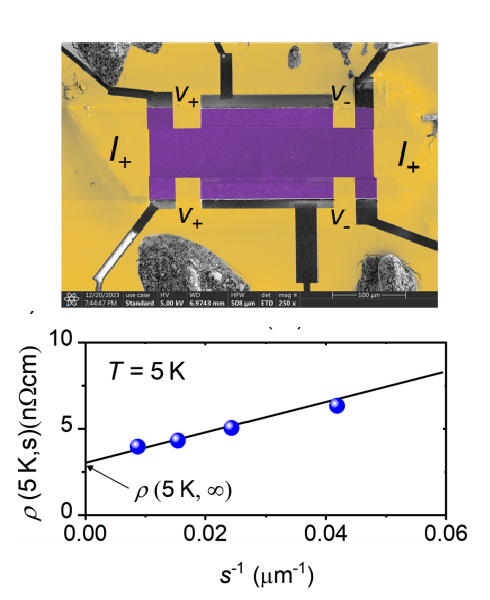
\includegraphics[width=0.49\linewidth]{fig1_sample.png}
		\figcap{Fig. 1}{Device and  effective width scaling}{%
			\textbf{(a)} False-colour SEM of the Cd Hall bar; current $I_{\pm}$ and voltage $V_{\pm}$ leads define the channel.Made by Focused Ion Beam (FIB)\textbf{(b)} At $T=5$\,K the resistivity is linear in $s^{-1}$: the intercept isolates the bulk term $\rho(5\,\mathrm{K},\infty)$, while the slope measures the boundary contribution.s is square root of width and thickness of the device (effective width)}
	\end{figurebox}
	\vspace{5pt}

	\begin{figurebox}\centering
		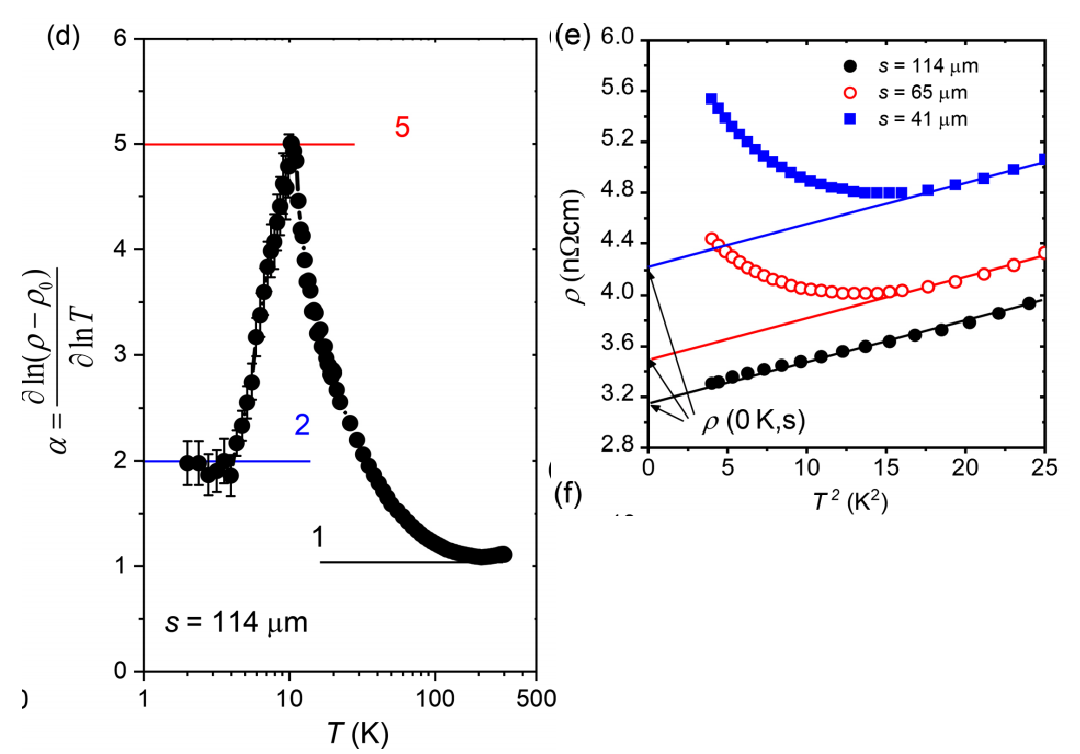
\includegraphics[width=0.71\linewidth]{fig2_diffusive.png}
		\figcap{Fig. 2}{  $T^2$ scaling for Diffusive Regime  }{%
			\textbf{(d)} For $s=114\,\mu$m(diffusive ), $\alpha=\partial\ln(\rho-\rho_0)/\partial\ln T$ plateaus at 2 (electron--electron scattering), peaks near 10\,K, then tends to 1 at high $T$(electron-phonon scattering). \textbf{(e)} $\rho$ versus $T^2$ for three widths: the zero-temperature offset $\rho(0\,\mathrm{K},s)$ grows as $s$ shrinks.For smaller device it deviates from the T square law}
	\end{figurebox}

	 	
	{\color{Line}\hrule height 0.5pt}\par
	\vspace{3pt}
	{\fontsize{10.6}{13.3}\selectfont
	A device's electron-transport regime is determined by its physical dimensions and by a competition between two different scattering mechanisms: momentum-relaxing collisions (with impurities or phonons), which decrease the total momentum of the electrons, and momentum-conserving collisions (between electrons), which merely exchange momentum among the electrons. When momentum-relaxing collisions dominate and the resulting electron mean free path is much smaller than the device width, transport is diffusive. When those momentum-relaxing collisions are less common, or if the device is very narrow, the mean free path is set by the device width, and transport is ballistic. An intermediate hydrodynamic regime occurs when momentum-conserving collisions are dominant, meaning that electrons collide with one another many times before losing momentum to the boundaries of the device or to other momentum-relaxing collisions (Fig.~1). In this regime, the electron fluid develops a parabolic velocity profile across the device's width, resulting in a conductivity that scales quadratically with width. The fluid's resistance to flow---its viscosity---is set by the interval between electron--electron collisions, which in a Fermi liquid is inversely proportional to $T^2/E_F$ (where $T$ is the temperature and $E_F$ is the Fermi energy) [5]. Warming the fluid or reducing $E_F$ increases the collision frequency and lowers its viscosity, causing conductivity to scale quadratically with temperature---the signature of the Gurzhi effect.\par}
\end{minipage}\hfill
\begin{minipage}[t]{0.36\textwidth}\vspace{0pt}\RaggedRight
	\fontsize{10.6}{13.3}\selectfont

	\begin{figurebox}\centering
		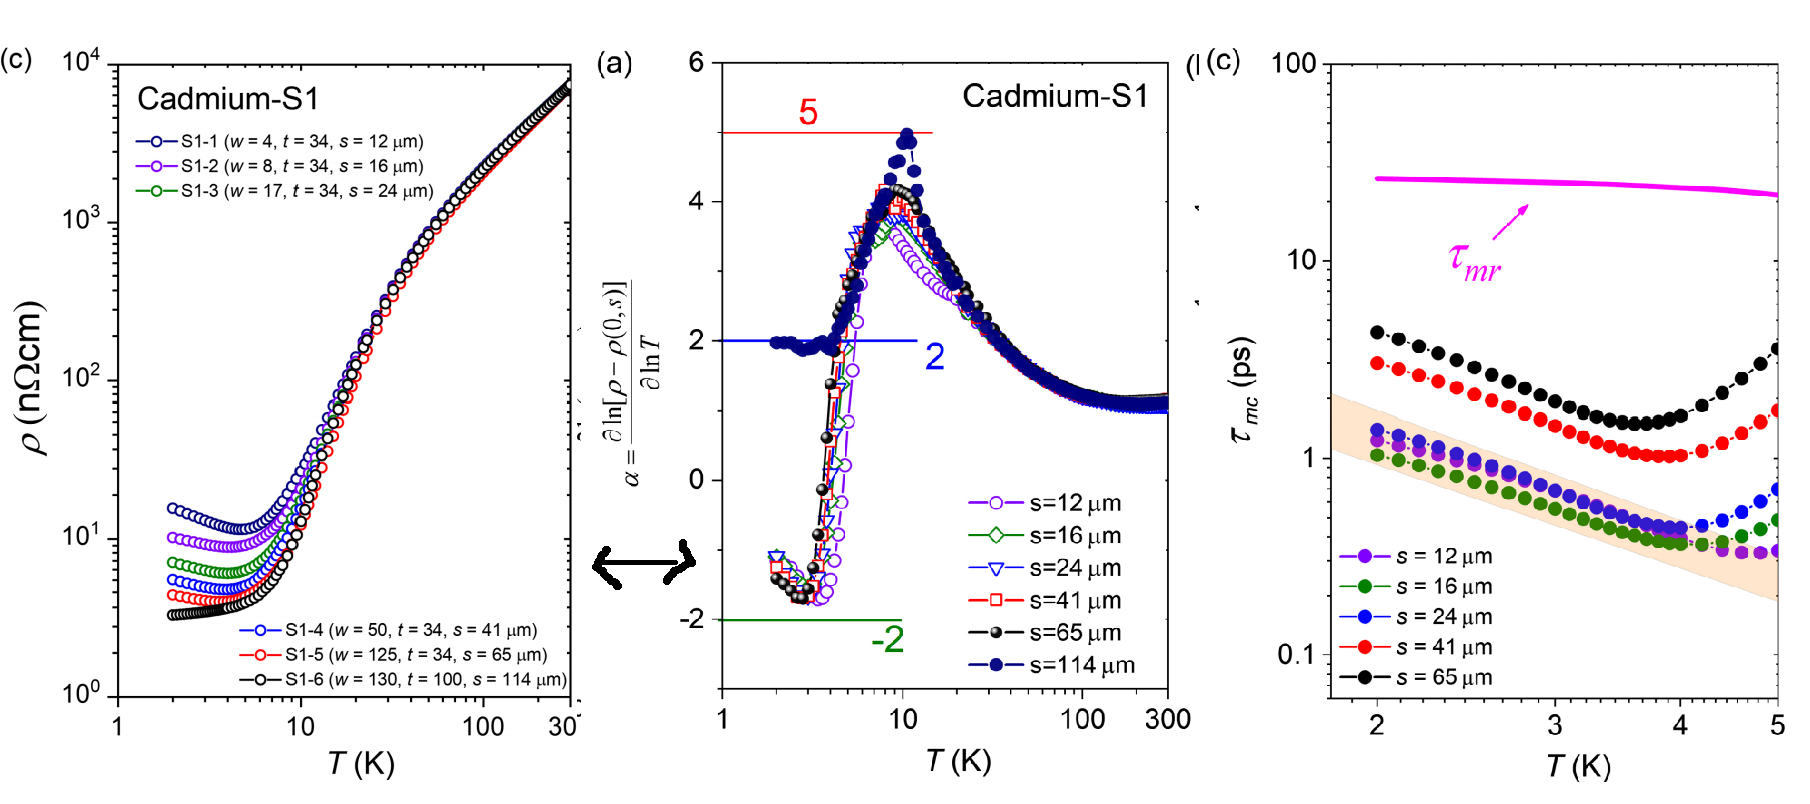
\includegraphics[width=1.00\linewidth]{fig3_hydrodynamic.png}
		\figcap{Fig. 3}{ $T^{-2}$ scaling for Hydrodynamic Regime  }{%
			\textbf{(c) and (a)} descibes the same thing .For smaller device in hydrodynamic regime the resistivity  behaves with  $T^{-2}$ law.(anomalous.Other assumptions including Anderson localization and 	Kondo impurity )
			\textbf{c }$\tau_{\mathrm{MR}}$ measured from the thickest sample.As the scale increases, the characteristic time of mc gradually approaches that of mr, moving from the hydrodynamic regime to the diffusive regime.}
	\end{figurebox}
	\vspace{5pt}

	\begin{figurebox}\centering
		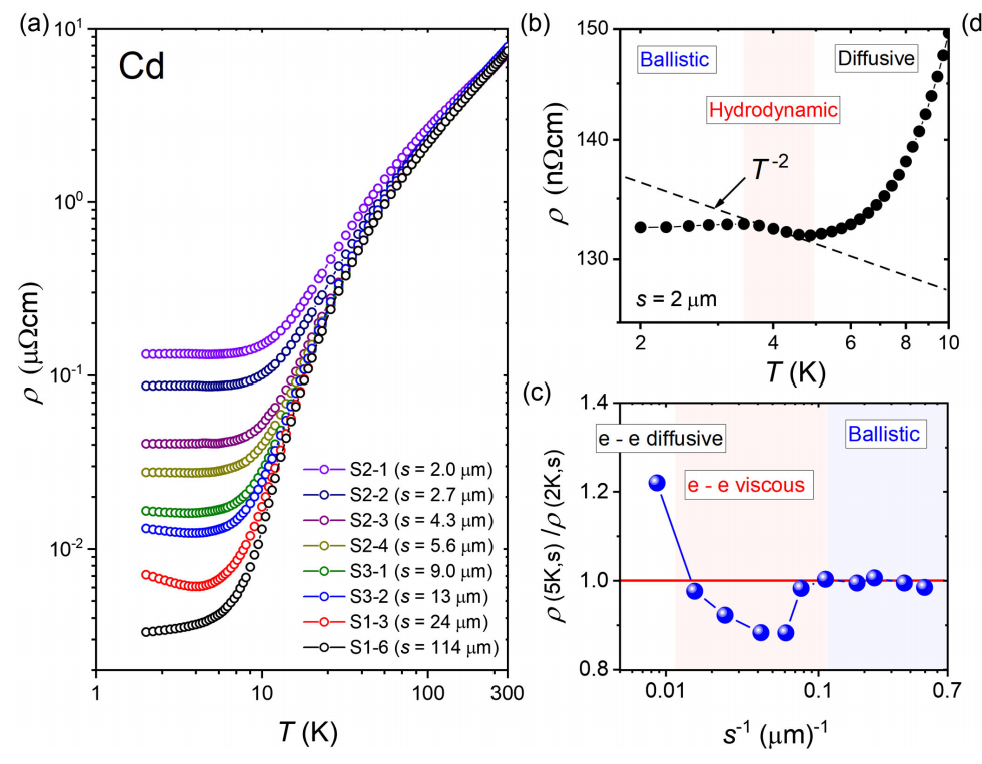
\includegraphics[width=0.89\linewidth]{fig4_ballistic.png}
		\figcap{Fig. 4}{ Ballistic Regime: independent of temperature}{%
			\textbf{(a)} $\rho(T)$ for Cd channels from $s=2$ to $114\,\mu$m. \textbf{(b)} fixed sample.As the temperature drops, the average free path becomes longer (diffusive $\rightarrow$ hydrodynamic $\rightarrow$ ballistic). for Cadmium,$\tau_{\mathrm{MR}}T^2$>$\tau_{\mathrm{MC}}T^2$  \textbf{(c)} $\rho(5\,\mathrm{K},s)/\rho(2\,\mathrm{K},s)$ crosses from electron--electron diffusive, through viscous, to ballistic as the channel narrows.}
	\end{figurebox}

		

 
	\sectionhead{Open questions}{My research notes}
	\begin{questionbox}
		 \begin{itemize}
		 \item By designing the geometric structure of the Fermi surface, we can make momentum-conserving collisions more efficient, rather than merely reducing impurity scattering?$\tau \propto \frac{ \hbar E_F}{(k_B T)^2}$
		 \item how to reconstruct the flow map of viscous electron fluid physically  ?2D cases?1D cases?
		 \item viscous electron fluid exist.How about high $R_e$ and turbulent electron?
		 \item strong -correlated electron fluid?
		 \end{itemize}
	\end{questionbox}
\end{minipage}

\vfill
{\color{Line}\hrule height 0.7pt}\par
\vspace{3pt}
{\smallnote{\textbf{PERSONAL RESEARCH NOTES} \quad Keep observations, author interpretations, and your own hypotheses distinct. \hfill Source panels: Figs.~1--4 \quad\textbullet\quad DOI: \href{https://doi.org/10.1103/g32f-j6q2}{10.1103/g32f-j6q2} \quad\textbullet\quad Confidence: preliminary / checked / revisit}}

\end{document}
